\section{Mind Refreshing SVM \hpoints{40}}

\begin{enumerate}
\item \textbf{Finite Features}: You are given the data set $D$ shown
  in in Figure~\ref{fig:svm_dataset} with data from a single feature
  $X_1$ in $\mathbb{R}^1$ and corresponding label $Y\in\{+,-\}$. The
  data set contains three positive examples at $X_1=\{-3,-2,3\}$ and
  three negative examples at $X_1=\{-1,0,1\}$.

  \begin{figure}[h]
    \begin{center}
      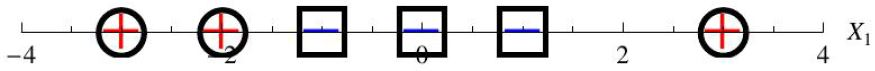
\includegraphics[width=4in]{images/svm_dataset.jpeg}
    \end{center}
    \caption{Dataset for SVM feature map task.}
    \label{fig:svm_dataset}
  \end{figure}
  
  This data set, \emph{in its current feature space}, cannot be
  perfectly separated using a linear separator.  The data changes
  class twice along only one dimension; a linear classifier in one
  dimension can only represent a single split.  In this problem, we'll
  investigate mapping the data to another feature space.

  \begin{enumerate}
  \item \points{2} Lets define the simple feature map
    $\phi(u)=(u,u^2)$ which transforms points in $\mathbb{R}^1$ to
    points in $\mathbb{R}^2$.  Apply $\phi$ to the data and plot the
    points in the new $\mathbb{R}^2$ feature space.
  
  \item \points{2} Can a linear separator perfectly separate the
    points in the new $\mathbb{R}^2$ features space induced by $\phi$?
    If so, draw a linear separator that works.  If not, explain why
    not.

   
  \item \points{4} Give the analytic form of the kernel that
    corresponds to the feature map $\phi$ in terms of only $X_1$ and
    $X_1^{\prime}$.  Specifically define $k(X_1,X_1^{\prime})$.
  
  \item \points{7} Construct a maximum-margin separating hyperplane.
    This hyperplane will be a line in $\mathbb{R}^2$, which can be
    parameterized by its normal equation, i.e. $w_1 Y_1 + w_2 Y_2 + c
    = 0$ for appropriate choices of $w_1,w_2,c$.  Here, $(Y_1,Y_2) =
    \phi(X_1)$ is the result of applying the feature map $\phi$ to the
    original feature $X_1$. Give the values for $w_1, w_2, c$.  Also,
    explicitly compute the margin for your hyperplane.  You do not
    need to solve a quadratic program to find the maximum margin
    hyperplane.  Instead, let your geometric intuition guide you.
  
  \item \points{4} On the plot of the transformed points (from part
    3), plot the separating hyperplane and the margin, and circle the
    support vectors.

  \item \points{2} Draw the decision boundary separating of the
    separating hyperplane, in the original $\mathbb{R}^1$ feature
    space.

  
  \item \points{4} Compute the coefficients $\alpha$ and the constant
    $b$ in \autoref{eqn:svm_form} for the kernel $k$ and the support
    vectors $SV=\{u_1,u_2\}$ you chose in part 6.  Be sure to explain
    how you obtained these coefficients.
    \begin{eqnarray}
      y(x) = \sign \left( \sum_{i=1}^{|SV|} \alpha_i y_i k(x, u_i) + b \right)
      \label{eqn:svm_form}
    \end{eqnarray}
    Think about the dual form of the quadratic program and the
    constraints placed on the $\alpha$ values.


  \item \points{2} If we add another positive ($Y=+$) point to the
    training set at $X_1=5$ would the hyperplane or margin change?
    Why or why not?
  \end{enumerate}
  
\item \textbf{Infinite Features Spaces and Kernel Magic}: Lets define
  a new (infinitely) more complicated feature transformation
  $\phi_n:\mathbb{R}^1 \rightarrow \mathbb{R}^n$ given in
  \autoref{eqn:phi}.
  \begin{eqnarray}
    \phi_n(x) = \left\{ e^{-x^2/2}, e^{-x^2/2} x, \frac{e^{-x^2/2}x^2}{\sqrt{2}},
    \ldots,
    \frac{e^{-x^2/2}x^i}{\sqrt{i!}}
    \ldots,
    \frac{e^{-x^2/2}x^n}{\sqrt{n!}}
    \right\}
    \label{eqn:phi}
  \end{eqnarray}
  Suppose we let $n \rightarrow \infty$ and define new feature
  transformation in \autoref{eqn:hilbert_vector}.  You can think of
  this feature transformation as taking some finite feature vector and
  producing an infinite dimensional feature vector rather than the
  simple two dimensional feature vector used in the earlier part of
  this problem.
  \begin{eqnarray}
    \phi_{\infty}(x) = \left\{ e^{-x^2/2}, e^{-x^2/2} x,
    \frac{e^{-x^2/2}x^2}{\sqrt{2}},
    \ldots,
    \frac{e^{-x^2/2}x^i}{\sqrt{i!}}
    \ldots
    \right\}
    \label{eqn:hilbert_vector}
  \end{eqnarray}
  
  \begin{enumerate}
  \item \points{3} Assuming a \emph{consistent} dataset, is there a
    finite set of points that cannot be linearly separated in this
    feature space?  If so, give an example dataset.  If not, explain
    why not.  Note: A consistent dataset is one where there aren't any
    points $\bx_i = \bx_j$ where $y_i \ne y_j$.  That is, no point can
    be labeled multiple different things.

  \item \points{4} We know that we can express a linear classifier
    using only inner products of support vectors in the transformed
    feature space as seen in \autoref{eqn:svm_form}.  It would be
    great if we could some how use the feature space obtained by the
    feature transformation $\phi_{\infty}$.  However, to do this we
    must be able to compute the inner product of examples in this
    infinite vector space.  Lets define the inner product between two
    infinite vectors $a=\{a_1,\ldots,a_i,\ldots\}$ and
    $b=\{b_1,\ldots,b_i,\ldots\}$ as the infinite sum given in
    \autoref{eqn:innerproduct_sum}.
    \begin{eqnarray}
      k(a,b) = a \cdot b = \sum_{i=1}^{\infty} a_i b_i
      \label{eqn:innerproduct_sum}
    \end{eqnarray}
    We cannot explicitly compute $k(a,b)$ in this form since it
    contains an infinite sum.  However, we can re-write $k(a,b)$ in a
    form that is efficiently computable.  Derive the efficiently
    computable form.  \emph{Hint}: You may want to use the Taylor
    series expansion of $e^x$ which is given in
    \autoref{eqn:taylorseries}.
    \begin{eqnarray}
      e^{x}=\lim_{n \rightarrow \infty} \sum_{i=0}^n \frac{x^i}{i!}
      \label{eqn:taylorseries}
    \end{eqnarray}

  \item \points{6}  Prove or disprove each claim below.
  
    \begin{enumerate}
    \item Suppose we translate the inputs $x'_i = x_i + x_0$ for some
      arbitrary $x_0$ before using the kernel above in an SVM.  Will my
      kernel function change? (i.e., does $k(x_i,x_j) = k(x'_i,x'_j)$)?
    \item What if we negated all the inputs $x'_i = -x_i$?
    \item What about rescaling $x_i' = ax_i$ for some positive scalar $a$?
      
      
    \end{enumerate}  
  \end{enumerate}
\end{enumerate}
  
\PointStats
